\subsubsection{Почему в УПТ получили широкое распространение дифференциальные каскады?}

Усилителями постоянного тока называют такие устройства, которые могут усиливать медленно изменяющиеся электрические сигналы. Они способны усиливать и переменные и постоянные составляющие входного сигнала. Усилители постоянного тока имеют много разновидностей. Т.к. такие устройства пропускают наряду с переменной составляющей еще и постоянную, то отдельные каскады должны быть связаны между собой либо непосредственно, либо через резисторы, но не через разделительные конденсаторы или трансформаторы, которые не пропускают постоянную составляющую.

Основной проблемой УПТ является т.н. \textbf{Дрейф нуля} - отклонение напряжения на выходе усилителя от начального(нулевого) значения при отсутствии входного сигнала. Основной причиной этого явления является температурная и временная нестабильность активных элементов схемы усилителя, резисторов, источников питания.

Одним из возможных путей уменьшения дрейфа нуля является использование дифференциальных усилителей.

\begin{center}
	\begin{figure}[h!]
		\center{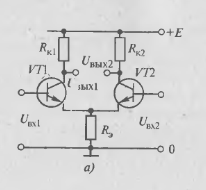
\includegraphics[scale=0.9]{DiffUs.png}}
		\caption{Схема}
	\end{figure}
\end{center} 

Дифференциальный усилительный каскад имеет два входа и усиливает разность напряжений, приложенных к ним. Если на оба входа подать одинаковое(синфазное) напряжение, то усиление будет чрезвычайно мало. Т.о., дифкаскад не усиливает синфазный сигнал. Дифференциальный каскад состоит из двух транзисторов, эмиттеры которых соединены и подключены к общему резистору $R_e$. Для сигнала $U_{in_1}$ транзистор VT1 включен по схеме с ОЭ, VT2 - с ОБ. Для второго сигнала симметрично.

На практике дифкаскады выполняют симметрично. Следовательно, мы можем предположить, что каскад абсолютно симметричен. В этом случае при равных входных сигналах токи транзисторов равны между собой. Пусть входные напряжения получат одинаковые приращения разных полярностей $\frac{1}{2}\Delta U_{in}$:
$$
U'_{in_1} = U_{in_1} + \Delta U_{in}/2
$$
$$
U'_{in_2} = U_{in_2} - \Delta U_{in}/2
$$ 

В результате ток одного транзистора увеличится на $\Delta I_K$, а другого на столько же уменьшится:
$$
I'_{K1} = I_{K1} + \Delta I_K
$$ 
$$
I'_{K2} = I_{K2} + \Delta I_K
$$ 

При этом результирующий ток через резистор $R_e$ останется без изменения. Постоянным будет и падение напряжения на нём. На выходе берут разность выходных сигналов $U_1 - U_2$. таким образом, т.к. один изменился в одну сторону, другой в другую, то результирующее изменение будет пропорционально $2\Delta I_K R_K$

В случае синфазного же сигнала, токи коллекторные получат одинаковые приращения => изменения выходного сигнала нет.Т.е. дифкаскад не усиливает синфазные сигналы.

Таким образом, дифференциальные усилители имеют очень низкий дрейф нуля и высокую степень подавления синфазных помех. Но при этом требуется высокая степень симметрии схемы.
